\section{System}\label{design}

\subsection{Development Environment}

I have developed my project to run on a Linux platform, and have used version 12.04 of the Ubuntu operating system during the system's development (Ubuntu, 2013 \cite{Ubuntu12LTS}). Interaction with the system is via the standard terminal. Appendix \ref{app:installation} details installation instructions for the necessary software packages and libraries for the project. The instructions assume the user is using an Internet-connected computer running a recent version of the Ubuntu operating system (v12.04 or above).

System-level software requirements include:

\begin{itemize}
    \item MySQL v5.5, Python v2.7, Virtualenv, NumPy, SciPy
\end{itemize}

Other dependencies are installed locally to the project.

\subsection{Data Migration}

\subsubsection{The Original Decanter Wines Database}

\begin{figure}[h!]
    \caption{Wines Database Represented as UML Class Diagram}
    \centering
        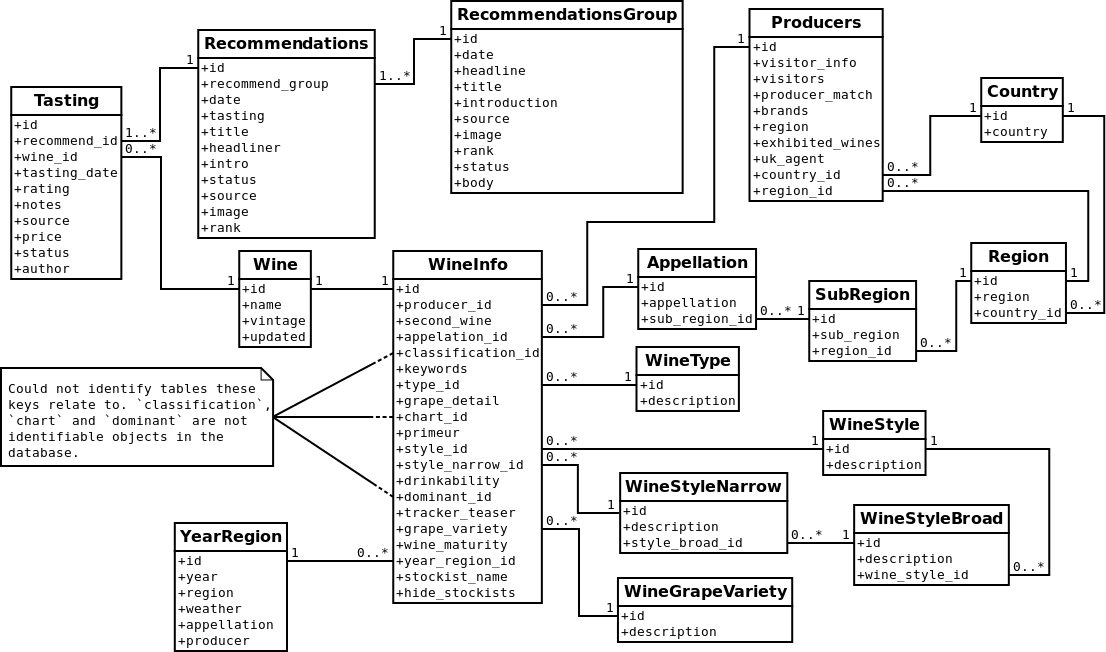
\includegraphics[width=14cm]{DecanterWineDB}
    \label{fig:decanterdb}
\end{figure}

The data source I have used for my project is the wines database belonging to Decanter.com \cite{DecanterWine}. The database contains nearly 40,000 professional ratings and tasting notes for wines from as far back as 1986, featuring vintages as far back as 1917.

I had hoped that the data would be fairly usable as it was received, as the data is currently used on the Decanter.com website, but on examination it was clear that there would be quite a lot of work to do in order to repurpose the data for my system.

I have modelled the database as a class diagram (Figure \ref{fig:decanterdb}). This diagram represents the 16 tables in the original database, the columns present in those tables, and the relationships between them.

One thing immediately apparent about the database is that there are circular relationship between some of the tables. For example, the table WineInfo contains foreign key fields for both WineStyleNarrow and WineStyle, but it is the case that a association with WineStyleNarrow already encompasses an association with WineStyle, via WineStyleNarrow's association with WineStyleBroad, which associates with WineStyle. Duplicating the association in this way makes the database difficult to maintain as there is a dependency between the two foreign keys style\_id and style\_narrow\_id on the WineInfo table which means that both must be updated any time that one is. There is a similar situation between the keys appellation\_id and producer\_id in the same table.

In addition to unnecessary duplication of associations in the WineInfo table there are foreign keys for missing, or unidentifiable, tables: classification\_id, chart\_id and dominant\_id. It is likely that these keys relate to tables removed from the database at one time or other.

The WineInfo table is a mixture of foreign keys joining to very small tables, such as type\_id joining to WineType, where WineType is a table holding only a single non-key field. This approach, of factoring out any non-integer fields to separate tables, is inconsistent with the fact that the same table also has several text fields, including second\_wine and tracker\_teaser. second\_wine only holds data in 450 of the 38762 entries in the table, and is an empty string by default in all others.

The problems with the database structure are consistent with the fact that the database has been developed over a long period of time in an ad hoc fashion. There have probably been many different developers, and the database, being many years old, has probably supported many incarnations of Decanter's website.

Despite the problems with the database I considered there to be a great deal of useful and interesting information in the database, with it to contain usable ratings and/or tastings for over 33,000 wines, but decided that it would be best to port it to a much more simple schema, and to strip out as much redundant data as possible, for the purposes of my project.

\subsubsection{The Cleaned-up Sommelier Development Database}

\begin{figure}[h!]
    \caption{Sommelier Database Represented as UML Class Diagram}
    \centering
        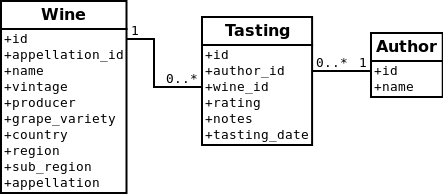
\includegraphics[width=10cm]{SommelierDBSimple}
    \label{fig:sommelierdb}
\end{figure}

For the new Sommelier database (Figure \ref{fig:sommelierdb}), I decided to minimise the complexity of the data, denormalizing the tables to make querying it as simple as possible. This would make updates to the data more complex, as any update to a field shared among many wines, for example a producer's name, would need to be replicated across a high number of records. As I did not intend to perform any writes on the data as part of my project I felt able to overlook this shortcoming of the design. If this system were to be applied in the real world, then there may be a need to refactor the database so that updates may be made more easily. 

As can be seen in Figure \ref{fig:sommelierdb}, I disregarded entirely much of the data from the original database. In many cases this was because I did not feel the data would be beneficial to my system. The Recommendations and RecommendationsGroup tables, for example, may have been useful, but the data in the tables was often incomplete and I did not reckon them to enrich the tasting notes enough to warrant migration. The fact that belonging to a certain group of recommendations may be used to infer similarities between wines seemed a tenuous reason to retain data in my development database.

The tables WineStyleNarrow and WineStyleBroad contained generic text descriptions for wine, such as ``rich and creamy'' and ``crisp and tangy''. I initially considered this to have potential for migration into tag data which I could reuse as part of my filtering. Unfortunately less than 6435 of the records in WineInfo had non-null values for their `style\_narrow\_id` field, and only 3397 of these had corresponding records in the Tasting table. This figure was only around 10\% of the number of wines I expected the Sommelier database to contain so I decided that the WineStyleNarrow and WineStyleBroad tables were not worth migrating.

The WineType table was ignored because no wines corresponded to it, there were values for `type\_id` in some WineInfo records, but none of those values corresponded with values in the `id` field in WineType.

Whatever the situation with the data in other tables, it was clear that the Tastings table would need to be at the centre of my system, as it is where user, item and rating are associated. Those are the core data points for most recommender systems, so I resolved that I would migrate all tastings which had both their `notes` and `rating` field populated, along with the associated authors and wines, to a new database using my simplified schema.

\subsubsection{The Author Problem}

\begin{table}[ht]
    \caption{Number of wines rated by each author}
    \centering
    \begin{tabular}{c c c}
        \\\hline\hline
        Author               & Wines tasted & Wines also tasted by other authors
        \\\hline
        Amy Wislocki         &           28 & 1  \\
        Andrew Jefford       &          105 & 38 \\
        Beverley Blanning MW &           13 & -  \\
        Carolyn Holmes       &            1 & -  \\
        Christelle Guibert   &          119 & 9  \\
        Clive Coates MW      &            6 & -  \\
        David Peppercorn     &           44 & -  \\
        Gerald D Boyd        &            7 & -  \\
        Harriet Waugh        &          250 & 23 \\
        James Lawther MW     &          226 & 21 \\
        John Radford         &            2 & -  \\
        Josephine Butchart   &           24 & 1  \\
        Norm Roby            &            4 & -  \\
        Rosemary George MW   &            6 & -  \\
        Serena Sutcliffe     &           31 & 15 \\
        Stephen Brook        &           19 & 3  \\
        Steven Spurrier      &          497 & 53 \\
        \\\hline
    \end{tabular}
    \label{table:authors}
\end{table}

\begin{table}[ht]
    \caption{Matrix of authors with wines tasted in common}
    \centering
    \begin{tabular}{c c c c c c c c c c}
        \\\hline\hline
        Author                   & SS & JL & JB & SB & CG & SS & HW & AJ & AW
        \\\hline
        Steven Spurrier (SS)     & -  & 6  & 1  & 1  & 7  & 0  & 15 & 30 & 1 \\
        James Lawther MW (JL)    & 6  & -  & 0  & 0  & 0  & 15 & 0  & 0  & 0 \\
        Josephine Butchart (JB)  & 1  & 0  & -  & 0  & 0  & 0  & 0  & 0  & 0 \\
        Stephen Brook (SB)       & 1  & 0  & 0  & -  & 0  & 0  & 1  & 1  & 0 \\
        Christelle Guibert (CG)  & 7  & 0  & 0  & 0  & -  & 0  & 1  & 5  & 0 \\
        Serena Sutcliffe (SS)    & 0  & 15 & 0  & 0  & 0  & -  & 0  & 0  & 0 \\
        Harriet Waugh (HW)       & 15 & 0  & 0  & 1  & 1  & 0  & -  & 10 & 0 \\
        Andrew Jefford (AJ)      & 30 & 0  & 0  & 1  & 5  & 0  & 10 & -  & 0 \\
        Amy Wislocki (AW)        & 1  & 0  & 0  & 0  & 0  & 0  & 0  & 0  & - \\
        \\\hline
    \end{tabular}
    \label{table:authormatrix}
\end{table}

The biggest shortcoming of the dataset is that the author of a tasting note is often not recorded. The number of tastings with known authors is only 1411, with there being only 18 named authors on the system. There are 25812 tastings with no author associated. I had reckoned on there being a much higher number of wine tastings with identifiable authors, given that each note and rating was always by a particular person. It appeared that this information had either not been entered, or had been lost.

Table \ref{table:authors} shows the distribution of tastings amongst authors, only 5 of which have tasted and rated more than 100 wines in the database. The table also shows how many of the wines tasted by each author have also been tasted and rated by other authors. Table \ref{table:authormatrix} shows the number of wines tasted in common for each of the authors (authors who have not tasted any wines in common with another author are omitted). It is clear that the data is extremely sparse. When migrating the data I was careful to ensure that I maintained all author to tasting associations, but rather than an oversight during migration, this shortcoming is inherent in the data. 

Measuring sparsity as the percentage of empty values in a matrix \textbf{M} of size $\vert \textit{A} \vert \times \vert \textit{W} \vert$, where \textit{A} is the vector of authors and \textit{W} is the vector of wines, we find that the database is 94\% sparse (Appendix \ref{app:datasparsity}). This is a worryingly sparse dataset for collaborative filtering. Su (2006 \cite{Su06}) reports a ``fast degradation of performance'' for the collaborative filtering algorithms they tested when the rate of sparsity exceeded 90\%. In addition there is the problem that ratings are not evenly distributed among authors, with a very small proportion of the authors accounting for the majority of ratings.

In a few cases there are tastings with no author associated where an author's initials or full name are recorded within the text of a tasting note, but unfortunately extracting and making use of these initials has been impractical given the time constraints of this project.

\subsection{Experimentation}

\subsubsection{Recommending Wines With Python}

\begin{table}[ht]
    \caption{Pearson Similarity of Authors (Appendix \ref{app:authorsim})}
    \centering
    \begin{tabular}{c c c c c c c c c c}
        \\\hline\hline
        Author                   & SS   & JL   & JB  & SB  & CG  & SS  & HW   & AJ   & AW
        \\\hline
        Steven Spurrier (SS)     & -    & 0.58 & 0.0 & 0.0 & 0.0 & -    & 0.67 & 0.49 & 0.0 \\
        James Lawther MW (JL)    & 0.58 & -    & -   & -   & -   & 0.22 & -    & -    & -   \\
        Josephine Butchart (JB)  & 0.0  & -    & -   & -   & -   & -    & -    & -    & -   \\
        Stephen Brook (SB)       & 0.0  & -    & -   & -   & -   & -    & 0.0  & 0.0  & -   \\
        Christelle Guibert (CG)  & 0.0  & -    & -   & -   & -   & -    & 0.0  & 0.0  & -   \\
        Serena Sutcliffe (SS)    & -    & 0.22 & -   & -   & -   & -    & -    & -    & -   \\
        Harriet Waugh (HW)       & 0.67 & -    & -   & 0.0 & 0.0 & -    & -    & 0.71 & -   \\
        Andrew Jefford (AJ)      & 0.49 & -    & -   & 0.0 & 0.0 & -    & 0.71 & -    & -   \\
        Amy Wislocki (AW)        & 0.0  & -    & -   & -   & -   & -    & -    & -    & -   \\
        \\\hline
    \end{tabular}
    \label{table:authormatrix}
\end{table}

In Chapter 2 of Collective Intelligence (Segaran, 2007 \cite{Segaran07}), Segaran details basic methods for user- and item-based collaborative filtering. Following the guidelines from this chapter I recreated Segaran's recommendation methods and applied them to my dataset, utilizing the Python command line interpreter (See code in Appendix \ref{app:recommendations}). 

Table \ref{table:authormatrix} shows the Pearson correlation between the authors. In cases where there are fewer than 3 items rated in common it is not possible for Pearson correlation to produce a useful result, and for such relationships my code returns a value of 0.0. Table \ref{table:authormatrix} shows that Pearson correlation was only able to produce similarity scores among five of the authors. For 18 authors in the system, recommendations could not be made at all for 13. This performance was consistent with my expectations given the sparseness of the data.

\subsection{API Interface}

\subsubsection{Interchange Format}

I chose to use JSON (JavaScript Object Notation) as my response format, which is a commonly used by RESTful APIs. It is designed to be natively handled by Javascript, but also has a sophisticated level of support in Python and other languages. 

\subsubsection{Routes}

For the API I conceived a very simple set of routes, based on providing accesss to two the different object types, authors and wines. with an additional index route at the root to aid discoverability. Figure \ref{api:routes} shows the routing structure for the API.

Each route has a very simple url structure, with the plural item type and page number accessing a paged list of items, and the item type and id accessing any individual item.

\begin{figure}
\footnotesize
\caption{API Routes. See code in Appendix \ref{app:flaskapp}}\label{api:routes}
\begin{verbatim}
/
/author/<id>
/authors/<page number>
/wine/<id>
/wine/<page number>
\end{verbatim}
\end{figure}
\normalsize

\subsubsection{Response Specification}

In principle RESTful services should favour discoverability, so as such the reponses contain links to other documents available on the API which are relevant to them. The objects are also designed to be consistent with each other as far as possible, using the same attribute for comparable properties wherever possible. 

Every response is an object with the attributes ``type'' and ``self''. The ``type'' attribute is to aid the client in interpreting the object and for this API can take the values ``author'', ``wine'', or ``list''. ``self'' is a sub-object containing at least the fields ``title'' and ``link'', with additional fields depending on the type of the object.

``wine''- and ``author''-type objects have the attribute ``related\_content'', which is where different kinds of recommended content will be inserted by the API. The ``list''-type objects have the attribute ``list'', which is a list of items with ``title'' and ``link'' attributes.

By structuring the responses this way I hope to make it as simple as possible for any client of the system to handle the different routes and navigate the API, as they should be able to ascertain the expected format of any object very quickly. 

This example represents the template of an object with the minimum required fields, where \%s represents a placeholder for a string value:

\footnotesize\begin{verbatim}
{
    ``type'': %s
    ``self'': {
        ``title'': %s
        ``link'': %s
    }
}
\end{verbatim}\normalsize

Full example responses for each content type are shown in Appendices \ref{app:apiindex}, \ref{app:apiauthors}, \ref{app:apiauthor}, \ref{app:apiwines}, and \ref{app:apiwine}. Responses are in the JSON format as specified by JSON.org (2013 \cite{JsonOrg}). 

\subsection{System Implementation}

Figure \ref{fig:sommelierclasses} is a UML class diagram representing the complete Sommelier system.

\begin{figure}[h!]
    \caption{Sommelier Class Diagram}
    \centering
        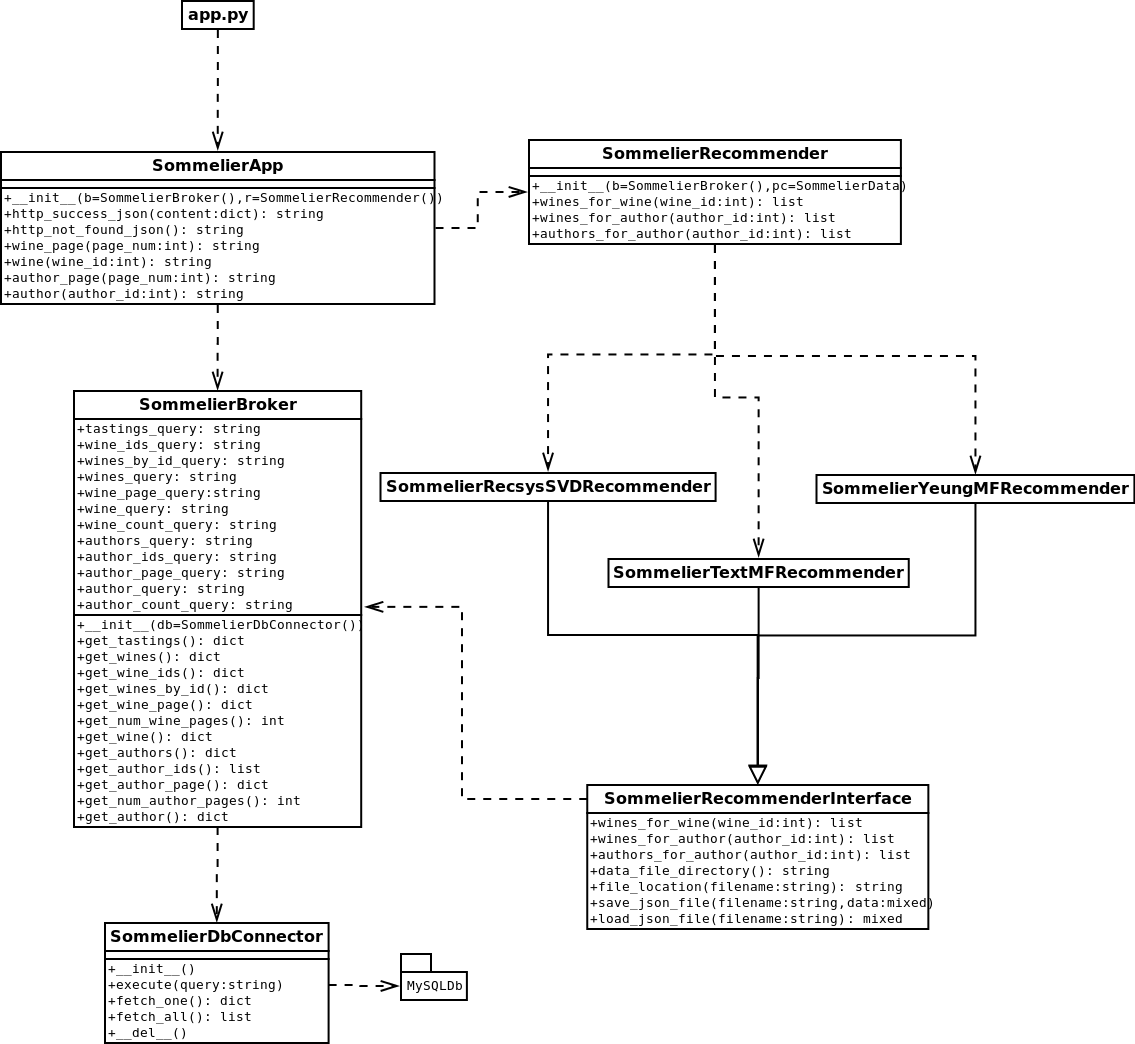
\includegraphics[width=15cm]{SommelierClassDiagram}
    \label{fig:sommelierclasses}
\end{figure}

The system is comprised of five main classes: Sommelier, SommelierBroker, SommelierDbConnector, SommelierRecommender, and SommelierRecommenderInterface. Additionally there are classes for different recommender implementations, and interactions with the files app.py and the sommelier\_precompute.py are indicated.

\subsubsection{Flask}

The Flask framework is initialized by the file app.py, and this file is where all HTTP requests to the API are handled. For each route there is configuration in this file that calls the corresponding method on Sommelier. In this way the workings of the Sommelier application are completely unknown to Flask, and similarly Sommelier does not need to manage requests or routing in any way. Flask simply receives a request and routes it appropriately, passing Sommelier's return values to its Response class, which formats the HTTP response in a standard manner.

The following example is the routing in app.py for the route /authors, and shows how the only coupling between the Flask and Sommelier systems is the one-to-one relationship of Flask routes to methods on Sommelier (line 6):

\footnotesize
\begin{verbatim}
@app.route('/authors', defaults = {'page_num': 1}, methods = ['GET'])
@app.route('/authors/<int:page_num>', methods = ['GET'])
def sommelier_authors(page_num):
    response_body, keyed_args_dict = sommelier.author_page(page_num)
    return Response(response_body, **keyed_args_dict)
\end{verbatim}
\normalsize

Flask has a built-in development server, which can be launched from app.py by calling app.run(). I do so in the main method, enabling debugging mode as a keyed argument:

\begin{verbatim}
if _name_ ==  '_main_':
    app.run(debug=True)
\end{verbatim}

By default this launches the server on port 5000 of localhost. Neither debug mode, not the development server are suitable for production environments, for which there are a number of other more robust options (Flask Deployment Options, 2013 \cite{FlaskDeployment}).

\subsubsection{Database Access}

Maintaining a connection to MySQL-python comes with the attendant complexity of managing of the lifecycle of a database connection object and cursor. To avoid having to recreate these objects many times in the code I wrote the wrapper SommelierDbConnector (see Figure \ref{fig:sommelierclasses}), which manages the connection and cursor in the minimum fashion, while exposing the minimum functionality to the application for executing on and fetching from the database. The full code is in Appendix \ref{app:sommelierdbconnector}.

To further abstract the database from the application logic of the system I created a broker class, SommelierBroker, which holds a hard coded set of queries that are performed on the database. I a new query is to be made on the system it is to be written into the broker. This approach has serious drawbacks, such as that it would be potentially unwieldy to scale. However, as I developed the system I found that there was only a very small set of queries that I was using, and decided that it was easier in the short term for one broker to own all of them.

\subsubsection{Recommenders}

The system gets recommendations via the facade class SommelierRecommender (see Figure \ref{fig:sommelierclasses}. This pattern abstracts away the complexity of making recommendations from the rest of the system, offering a simple interface with which to query whichever of the recommenders is instantiated. 

This pattern was very helpful when it came to developing the recommenders, as it makes it trivial to swap one out for another in the system.

\subsubsection{Precomputation}

For various recommendation approaches it is necessary to precompute data. I have not modelled this behaviour in Figure \ref{fig:sommelierclasses} as there are many potential ways of doing so. I have assumed that arbitrary scripts would be created and run on a scheduled basis to carry out precomputation for methods such as matrix factorization or SVD, where imputing matrices cannot practically be done at runtime.

